\documentclass[english,serif,mathserif,xcolor=pdftex,dvipsnames,table]{beamer}
\usetheme{gc3}

\usepackage[T1]{fontenc}
\usepackage[utf8]{inputenc}
\usepackage{babel}

\usepackage{gc3}

\title[Introduction]{%
  Overview of common GC3Pie use cases
}
\author[R. Murri, S3IT UZH]{%
  Riccardo Murri \texttt{<riccardo.murri@uzh.ch>}
  \\[1ex]
  \emph{S3IT: Services and Support for Science IT}
  \\[1ex]
  University of Zurich
}
\date{November~14--17, 2016}

\begin{document}

% title frame
\maketitle

\begin{frame}
  \frametitle{What is GC3Pie?}
  GC3Pie is \ldots
  \begin{enumerate}
  \item \alert<1>{An \emph{opinionated} Python framework for defining and running computational workflows;}
  \item A \emph{rapid development toolkit} for running user applications on clusters and IaaS cloud resources;
  \item The worst name ever given to a middleware piece\ldots
  \end{enumerate}

  \+
  As \emph{developers}, \alert<1>{you're mostly interested in this part.}
\end{frame}


\part{Uses of GC3Pie}

\begin{frame}[fragile]
  \frametitle{Uses of GC3Pie: parameter sweep}

  You have a simulation code that is dependent on a number of parameters.

  \+
  Run the code for all possible combinations of parameters.

  \+
  Then collect all the outputs and post-process to get a
  statistical overview.
\end{frame}


\begin{frame}[fragile]
  \frametitle{Uses of GC3Pie: model calibration}

  You have a simulation code that is dependent on a number of parameters.

  \+
  Run the code for all possible combinations of parameters, and
  find the ones that ``best'' approximate a given experimental result.
\end{frame}


\begin{frame}[fragile]
  \frametitle{Uses of GC3Pie: parallel processing}

  Run the same program over and over again,
  feeding it different input files each time.

  \+
  Then collect all the outputs and post-process to get a
  statistical overview.
\end{frame}


\begin{frame}[fragile]
  \frametitle{Uses of GC3Pie: parallel processing}
  (At times, you chop a large input file into pieces and process each one separately instead.)

  \+
  \begin{quote}
    ``For example, say we have a de novo assembly of 100,000
    contigs. If we run 1 BLAST job against NR it could take as long as
    50,000 minutes/35 days!! (30sec/query sequence), however if we
    split this job into subsets of 5,000 sequences and ran 20 jobs in
    "parallel" on a cluster, our total run-time is reduced to only 41
    hours.''
  \end{quote}
  \begin{references}
    \url{http://sfg.stanford.edu/BLAST.html}
  \end{references}
\end{frame}


\begin{frame}
  \frametitle{Uses of GC3Pie: workflows}

  \begin{center}
    Orchestrate execution of several applications:
    some steps may run in parallel, some might need to be sequenced.

    \+
    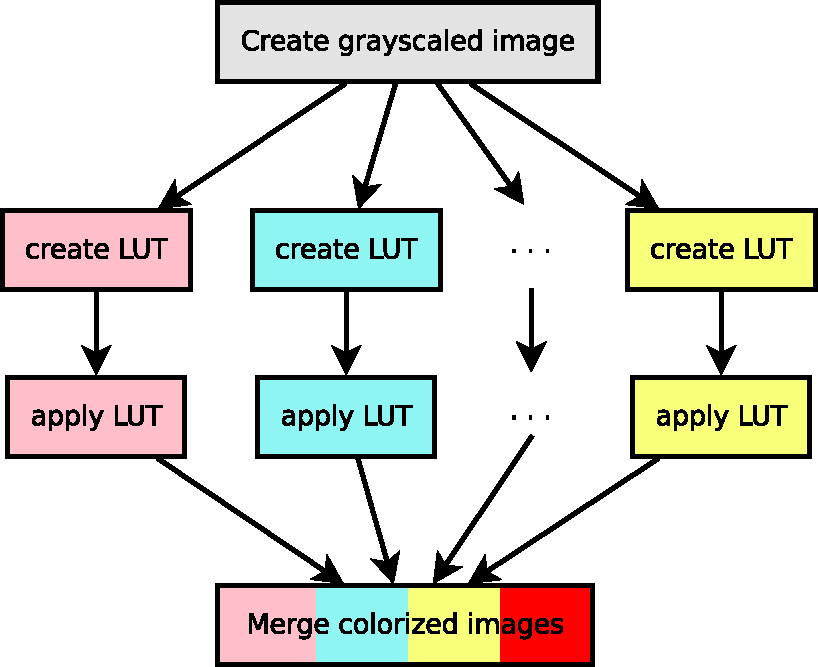
\includegraphics[width=0.70\textwidth]{fig/warholize-wkf.pdf}
  \end{center}
\end{frame}


\part{How GC3Pie works}

\begin{frame}
  \frametitle{A typical high-throughput script structure}

  \begin{enumerate}
  \item Initialize computational resources
  \item Prepare programs and inputs for submission
  \item Submit tasks
  \item Monitor task status (loop)
  \item Retrieve results
  \item Postprocess and display
  \end{enumerate}
\end{frame}


\newcommand<>\fullgraphicsframe[1]{%
  {
    \usebackgroundtemplate{\includegraphics[width=\paperwidth]{#1}}
    \begin{frame}[plain]
      % empty frame -- the graphics comes from above
    \end{frame}
  }
}

\fullgraphicsframe{fig/gc3pie-running-1.pdf}

\fullgraphicsframe{fig/gc3pie-running-3.pdf}

\fullgraphicsframe{fig/gc3pie-running-2.pdf}


\begin{frame}
  \frametitle{What GC3Pie handles for you}

  \begin{enumerate}\small
  \item Resource allocation (e.g. starting new instances on
    ScienceCloud)
  \item Selection of resources for each application in the session
  \item Data transfer (e.g. copying input files in the new instances)
  \item Remote execution of the application
  \item Retrieval of results (e.g. copying output files from the
    running instance)
  \item De-allocation of resources
  \end{enumerate}

\end{frame}


\end{document}

%%% Local Variables:
%%% mode: latex
%%% TeX-master: t
%%% End:
